\documentclass[a4paper,12pt]{book}
\setcounter{tocdepth}{3}
\setcounter{secnumdepth}{3}
\usepackage{lipsum}
%\usepackage[utf8]{inputenc}
%\usepackage{graphicx}
\usepackage{amsmath}
\usepackage{amssymb}
\usepackage{physics}
\usepackage{tcolorbox}
\usepackage{color}   %May be necessary if you want to color links
\usepackage{hyperref}
\usepackage{mathtools}
%\hypersetup{
%	colorlinks=true, %set true if you want colored links
%	linktoc=all,     %set to all if you want both sections and subsections linked
%	linkcolor=blue,  %choose some color if you want links to stand out
%	linktocpage
%}
\begin{document}

\author{Pugazharasu}
\title{Mathematical Physics}
\date{July 2020}

\frontmatter
\maketitle
\pagebreak
\chapter*{Preface}
This document is simply the collective summary of all of the fundamental mathematics that I have learnt over the years. This assumes a little mathematical maturity. More niche subjects such as analysis, topology and Lie theory are relegated in separate documents. This should only be treated as a revision/recall document and not as a learning material since it is devoid of lenghty explanations and often assumes you have at least briefly read through the cited texts or similar material.
\nopagebreak
\tableofcontents


%\pagebreak

\addcontentsline{toc}{chapter}{Preface}

\mainmatter
%\chapter{Logic}

%\chapter{Set Theory}

%\chapter{Categories}
This chapter is a summary of \cite{arxivmath}
%\chapter{Basics}
\section{Definitions}
\begin{itemize}
\item A Graph is a set of objects and the relationships between pairs of objects
\item A Graph $G(V,E)$, is a set of V \textbf{Vertices/nodes} and $E$ \textbf{Edges}
\end{itemize}
\begin{figure}[h]
	\centering
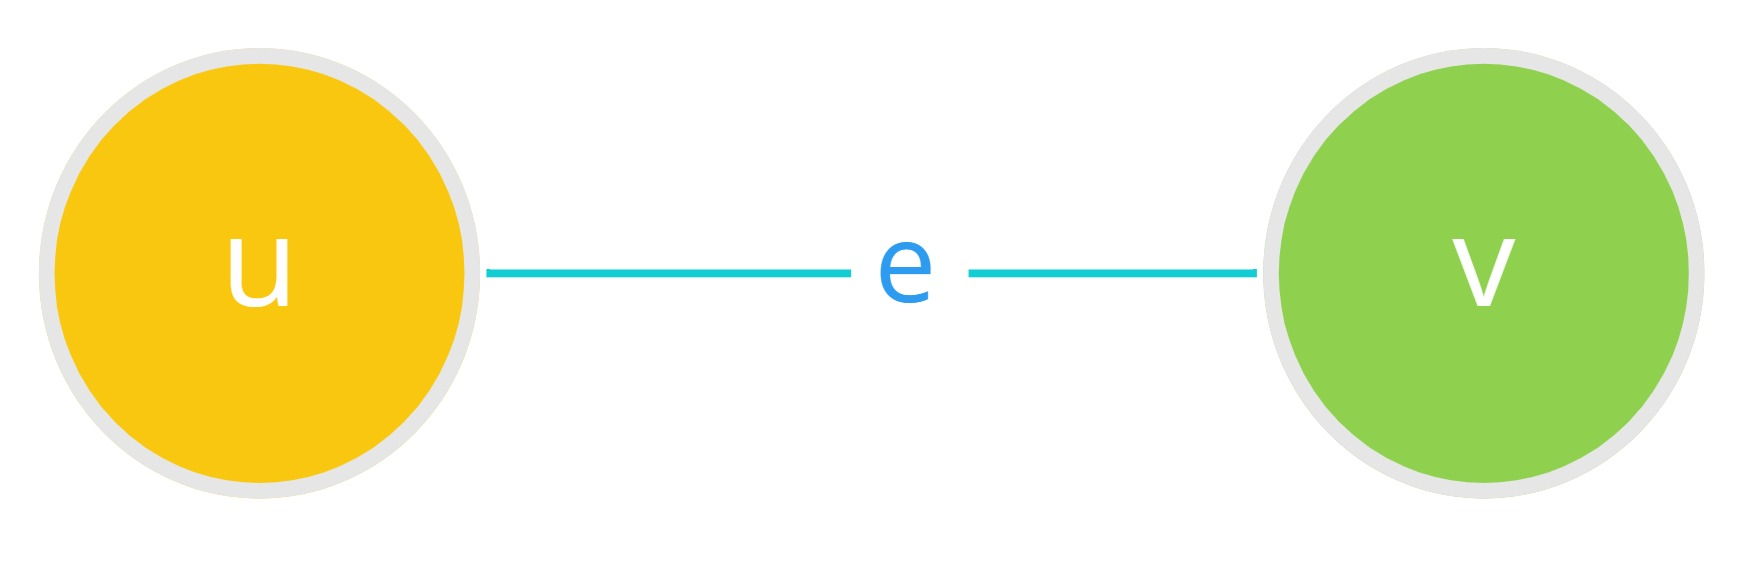
\includegraphics[scale = 0.1]{1.png}
\caption{A visual representation of a simple Graph}
\end{figure}
\begin{itemize}
\item For the above figure we say that:
\begin{itemize}
\item $e$ \textbf{Connects} $u$ and $v$
\item $u$ and $v$ are \textbf{End Points} of $e$
\item $u$ and $e$ are \textbf{Incident}
\item $u$ and $v$ are \textbf{Adjacent}
\item $u$ and $v$ are \textbf{Neighbors}
\end{itemize}
\item Or in set theory lingo as $G(\{u,v\},\{e\})$
\end{itemize}
\begin{figure}[h]\label{fig_2}
	\centering
	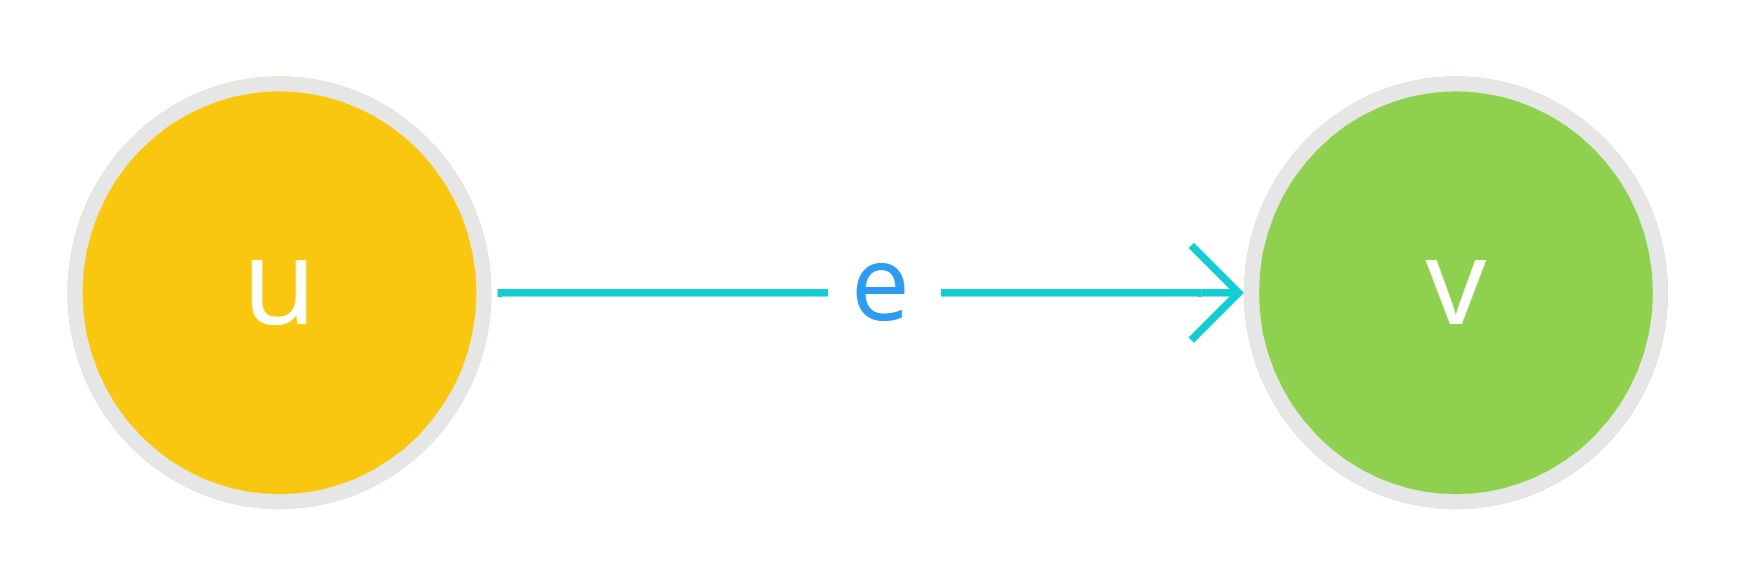
\includegraphics[scale = 0.1]{2.png}
	\caption{A visual representation of a simple directed Graph. Here $u$ is called the \textbf{tail} and $v$ the \textbf{head}}
\end{figure}
\begin{itemize}
\item There also exist \textbf{directed Edges/Arcs} i.e. , they describe asymmetric relations
\item Adding \ref{fig_2} to another directed graph with the same vertices but the edge pointing in the other direction results in a non-directed graph
\item \textbf{Degree} of a vertex is the number of its incident edges i.e. neighbours denoted by $deg(v)$
\item The degree of a graph is the maximum degree of its vertices
\end{itemize}
\section{Types of Graph}
\begin{itemize}
\item A \textbf{Regular graph} is a graph where each vertex has the same degree
\item A regular graph of $n$ degrees is called $n-$Regular
\item  The Complement of a graph $G = (V, E)$ is a graph $\bar{G} = (V, \bar{E})$ on the same set of vertices $V$ and the following set of edges:
\begin{itemize}
\item Two vertices are connected in $\bar{G}$ $\ iff$ they are not connected in $G$ i.e. $(u,v) \in \bar{E} \ iff \  (u,v) \notin E$
\item A \textbf{Path} is a continuous sequence of edges that connect two vertices
\item A \textbf{Walk} in a graph is a sequence of edges, such that each edge except for the first one starts with a vertex where the previous edge ended
\item The \textbf{Length} of a walk is the number of edges in it
\item A \textbf{Path} (rigorously) is a walk where all edges are distinct
\item A \textbf{Simple Path} is a walk where all vertices are distinct
\end{itemize}
\item  A \textbf{Cycle} in a graph is a path whose first vertex is the same as the last one; In particular, \textit{all the edges in a Cycle are
	distinct}
\item A \textbf{Simple Cycle} is a cycle where all vertices
except for the first one are distinct and
there first vertex is taken twice
\item A graph is called \textbf{Connected} if there is a path
between every pair of its vertices
\item  A \textbf{Connected Component} of a graph $G$ is a
maximal connected subgraph of $G$ i.e., a connected subgraph of $G$ which is not
contained in a larger connected subgraph of $G$
\item The \textbf{Indegree} of a vertex $v$ is the number of
edges ending at $v$
\item The \textbf{Outdegree} of a vertex $v$ is the number of
edges leaving $v$
\item A \textbf{Weighted Graph} associates a \textit{weight} with
every edge
\item The \textbf{Weight} of a path is the sum of the
weights of its edges
\item A \textbf{Shortest Path} between two vertices is a
path of the minimum weight
\item The \textbf{Distance} between two vertices is the
length of a shortest path between them
\end{itemize}
\begin{itemize}
\item A \textbf{Path Graph} $P_{n} \ \forall \ n \geq 2$, has $n$ vertices labeled $v_{n}$ and $n-1$ edges $\{v_{n-1}, v_{n}\}$
\end{itemize}
\begin{figure}[h]\label{fig_3}
	\centering
	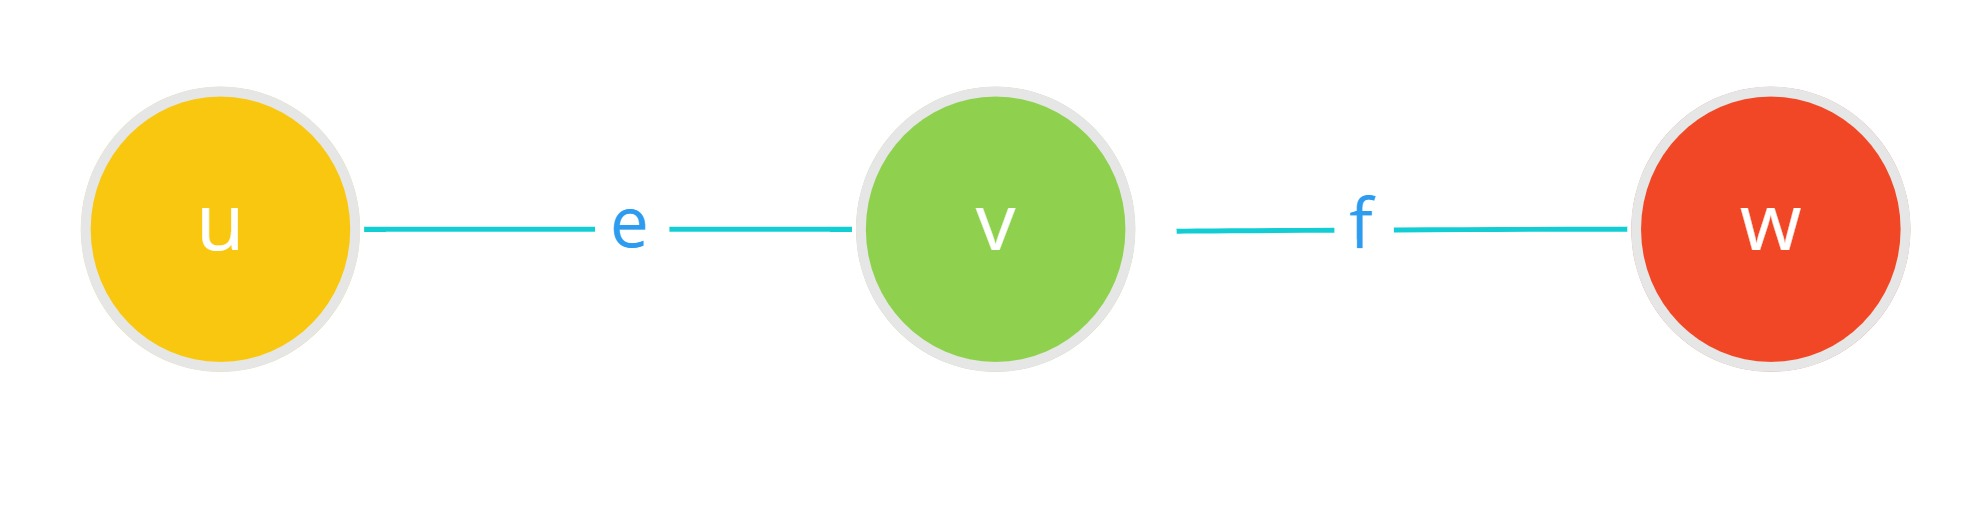
\includegraphics[scale = 0.1]{3.png}
	\caption{The Path Graph $P_{3}$}
\end{figure}
\begin{itemize}
\item A \textbf{Cycle Graph} $C_{n} \ \forall \ n \geq 3$, has $n$ vertices labeled $v_{n}$ and $n$ edges $\{v_{n-1}, v_{n}\},\{v_{n}, v_{1}\}$
\end{itemize}
\begin{figure}[h]\label{fig_4}
	\centering
	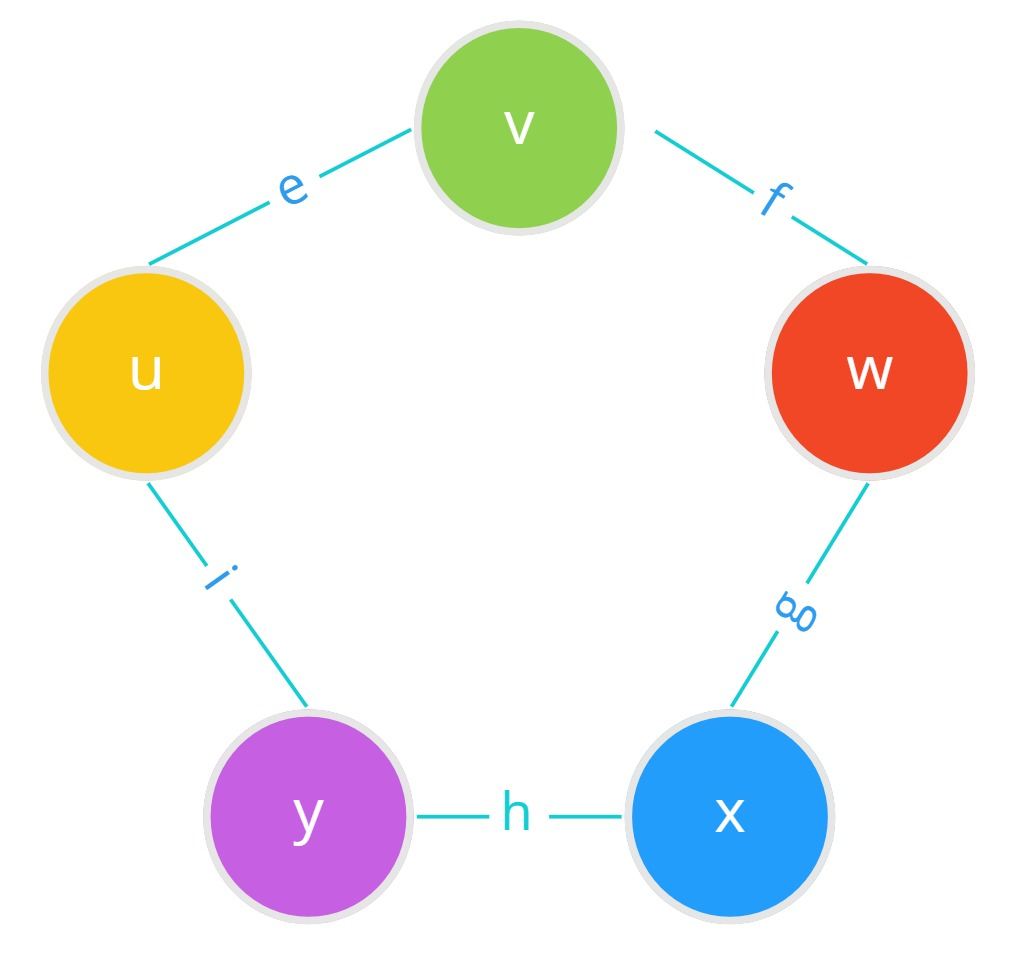
\includegraphics[scale = 0.2]{4.png}
	\caption{The Cycle Graph $C_{5}$}
\end{figure}
\pagebreak
\begin{itemize}
	\item A \textbf{Complete Graph (a.k.a Clique)} $K_{n} \ \forall \ n \geq 2$, has $n$ vertices labeled $v_{n}$ and all edges between them (i.e. $n(n-1)/2$ edges )
\end{itemize}
\begin{figure}[h]\label{fig_5}
	\centering
	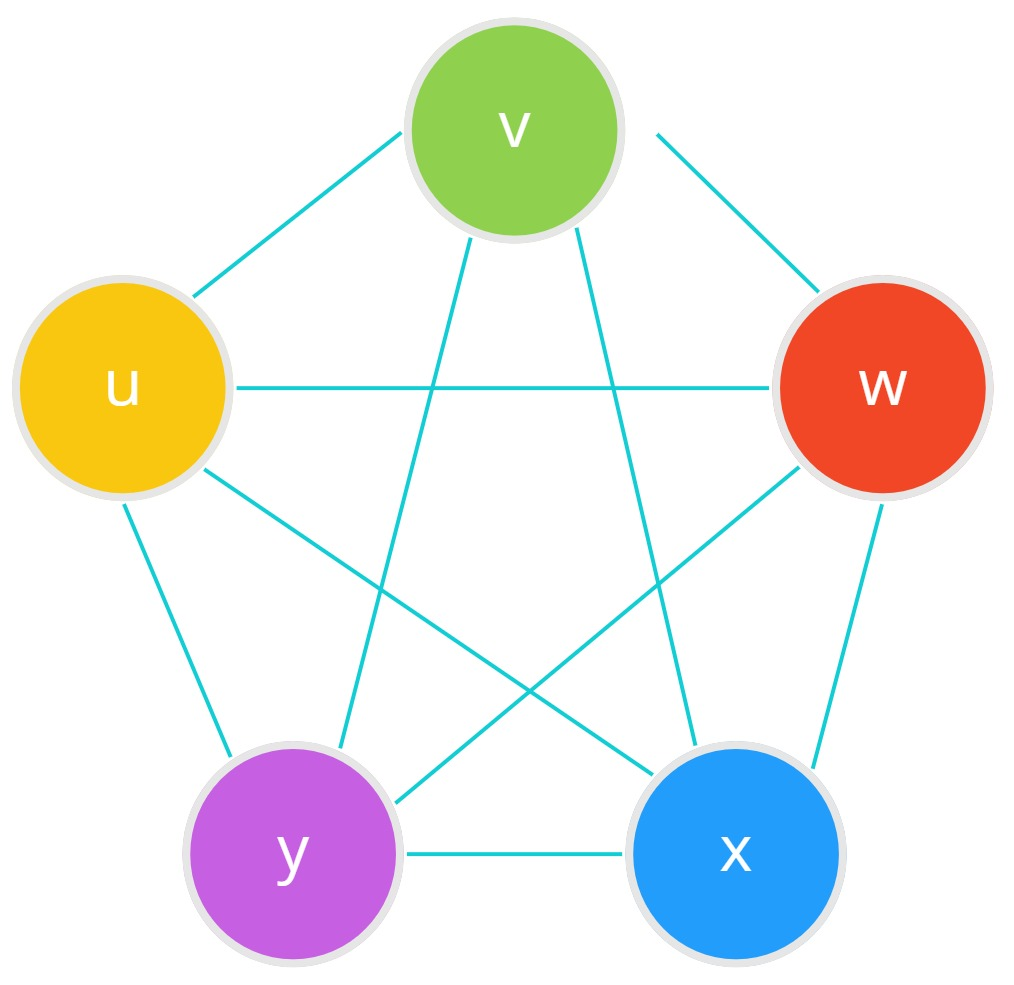
\includegraphics[scale = 0.2]{5.png}
	\caption{The Clique Graph $K_{5}$}
\end{figure}
\section{Trees}
\begin{itemize}
\item A tree is a connected graph without cycles
\item A tree is a connected graph on $n$ vertices with $n - 1$ edges
\item A graph is a tree if and only if there is a unique simple path between any pair of its vertices
\end{itemize}
\subsection{How to make a tree?}
\section{Bipartite Graphs}
\begin{itemize}
\item A graph $G$ is \textbf{Bipartite} if its vertices can be partitioned into two disjoint sets (sets with no common elements) $L$ and $R$ such that every edge of $G$ connects a vertex in $L$ to a vertex in $R$  i.e., no edge connects two vertices from
the same part
\item $L$ and $R$ are called the parts of $G$
\item Trees are Bipartite Graphs
\end{itemize}
\subsection{Examples and counter examples}
\begin{figure}[h]\label{fig_2}
	\centering
	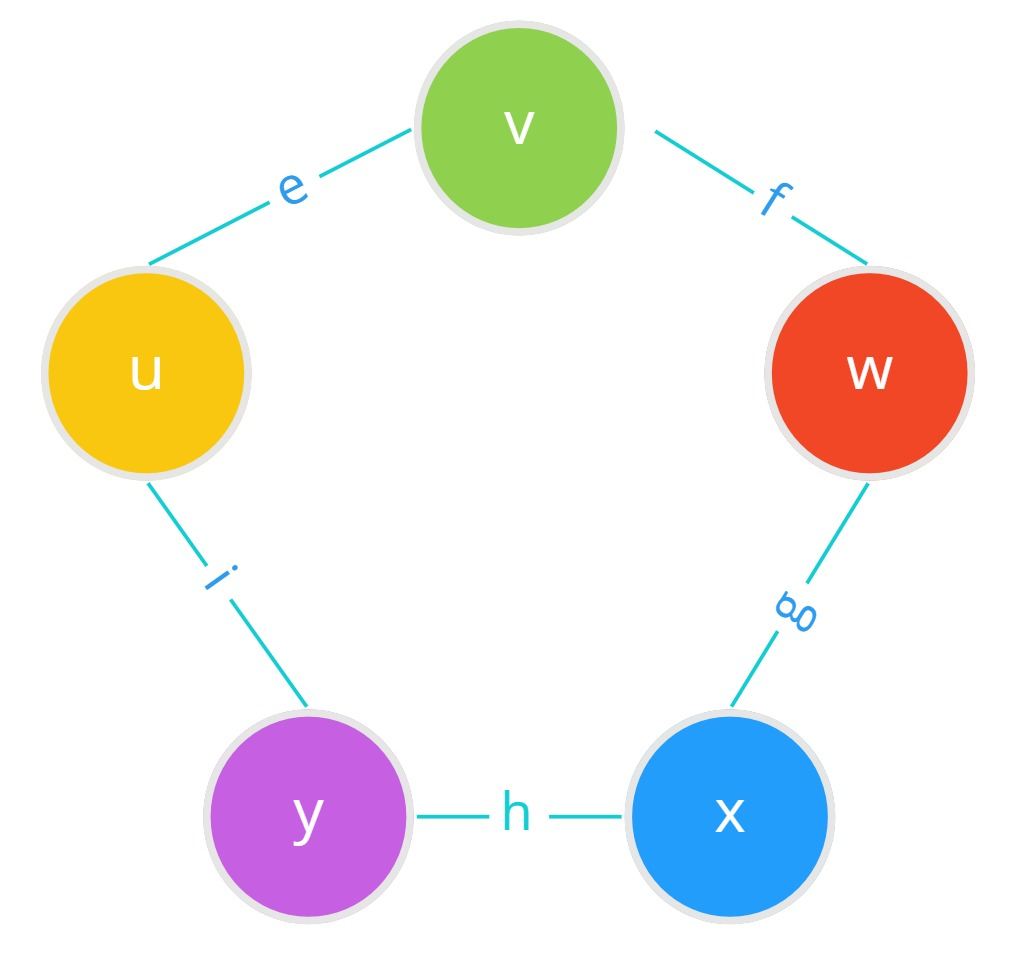
\includegraphics[scale = 0.1]{4.png}
	\caption{$C_{5}$ is not bipartite. In general, for odd $n > 2$, $C_{n}$ is not bipartite. However, }
\end{figure}

%
%\chapter{Groups}
This chpater is a summary of \cite{Nathan}, Chapters 2, 5, 6, 7, 8 and 9 from \cite{Artin}, Chapter 2 from \cite{Stillwell} and chapters 1 and 2 from 
\section{What is a group?}
A group is a system/algebraic structure that consists of a collection of actions/a set and an operator/binary operator to combine actions satisfying certain axioms (see below), in such a way that the result of two actions combined using a the operator is yet another action in the set.
\subsection{Group "Rules"}
\begin{enumerate}
	\item There is a predefined list of actions that never changes.
	\item Every action is reversible.
	\item Every action is deterministic.
	\item Any sequence of consecutive actions is also an action
\end{enumerate}
\subsection{Group Axioms}
A group is an algebraic structure $(\mathcal{G},\circ)$ which satisfies the following four conditions:
\begin{enumerate}
	\item \textbf{Closure:} $\forall \ a,b \in \mathcal{G}: a \circ b \in \mathcal{G}$ 
	\item \textbf{Associativity:} $\forall \ a, b, c \in \mathcal{G}: a \circ (b \circ c)  = (a \circ b) \circ c $   	  
	\item \textbf{Identity:} $\exists \ e \in \mathcal{G}: \forall \ a \in \mathcal{G}: e \circ a = a = a \circ e $
	\item \textbf{Inverse:} $ \forall \ a \in \mathcal{G}: \exists \  b \in \mathcal{G}: a \circ b = e = b \circ a$  	  %∀a∈G:∃b∈G:	a∘b=e=b∘a
\end{enumerate}
\section{What do groups look like?}
\subsection{Mapmaking}
\subsection{Mapping a group}
\subsection{Cayley diagrams}
\subsection{A touch more abstract}

\section{Why study groups?}
\subsection{Groups of symmetries}
\subsection{Groups of actions}
\subsection{Examples}

\section{Group Algebra}
\subsection{Multiplication tables}
\subsection{The classic definition}

\pagebreak

\section{Five families}
\subsection{Cyclic groups}
\subsection{Abelian groups}
\subsection{Dihedral groups}
\subsection{Symmetric groups}
\subsection{Alternating groups}

\section{Subgroups}
\subsection{Multiplication tables and Cayley diagrams}
\subsection{Seeing subgroups}
\subsection{Revealing subgroups}
\subsection{Cosets}
\subsection{Lagrange's theorem}

\section{Products and quotients}
\subsection{The direct product}
\subsection{Semidirect products}
\subsection{Normal subgroups and quotients}
\subsection{Normalizers}
\subsection{Conjugacy}

\section{The power of homomorphisms}
\subsection{Embeddings}
\subsection{Quotient maps}
\subsection{The Fundamental Homomorphism Theorem}
\subsection{Modular arithmetic}
\subsection{Direct products and relatively prime numbers}
\subsection{The Fundamental Theorem of Abelian Groups}
\subsection{Semidirect products revisited}

\pagebreak

\section{Sylow theory}
\subsection{Group actions}
\subsection{Approaching Sylow: Cauchy's Theorem}
\subsection{p-groups}
\subsection{Sylow Theorems}



\chapter{Rings}
\section{Definition}
\section{Formal Construction of Integers and Polynomials}

\chapter{Galois Theory}
\section{Heuristics}
\subsection{The big question}
\subsection{More big questions}
\subsection{Visualizing field extensions}
\subsection{Irreducible polynomials}
\subsection{Galois groups}
\subsection{The heart of Galois theory}
\subsection{Unsolvability}
\section{The Main Theorem of Galois Theory}
\section{Cubic Equations}
\section{Symmetric Functions}
\section{Primitive Elements}
\section{Proof of the Main Theorem}
\section{Quartic Equations}
\section{Kummer Extensions}
\section{Cyclotomic Extensions}
\section{Quintic Equations}

\include{./TeX_files/chapter06}
\include{./TeX_files/chapter07}
\include{./TeX_files/chapter08}
\chapter{Unconstrained Optimization \& Linear Programming}
\section{Basic Concepts}

\section{Linear Programming}
\section{Simplex Method}
\subsection{Simplex Method: Difficulties}

\chapter{Graphs \& Combinotorial Optimization}
\section{Combinotorial Optimization} 
Combinotorial Optimization concerns optimization problems of a discrete or combinatorial strcuture. It uses graphs and digraphs as basic tools.
\section{Graphs}

\section{Digraphs}
\section{Shortest Path Problems}
\subsection{Complexities}
\section{Bellman's Principle}
\section{Dijkstra's Algorithm}
\section{Shortest Spanning Trees}
\subsection{Greedy's Algorithm}
\subsection{Prim's Algorithm}
\section{Flows in Networks}
\subsection{Maximum Flow: Ford-Fulkerson Algorithm}
\section{Bipartite Graphs}

\chapter{Probability}
\section{Venn Diagrams}
\section{Probability}
\section{Permutations and Combinations}
\section{Random Variables and Distributions}
\section{Properties of Distributions}
\section{Functions of Random Variables}
\section{Generating Functions}
\section{Important Discrete Distributions}
\section{Important Continuous Distributions}
\section{The Central Limit Theorem}
\section{Joint Distributions}
\section{Properties of Joint Distributions}
\section{Generating Functions for Joint Distributions}
\section{Important Joint Distributions}

\chapter{Statistics}

\backmatter
\begin{thebibliography}{9}
	\bibitem{arxivmath}
	Jean Claude Dutailly.
	\textit{Mathematics for theoretical physics}.
	arXiv:1209.5665v2
	
	\bibitem{latexcompanion} 
	Michel Goossens, Frank Mittelbach, and Alexander Samarin. 
	\textit{The \LaTeX\ Companion}. 
	Addison-Wesley, Reading, Massachusetts, 1993.
	
	\bibitem{Nathan} 
	Nathan Carter 
	\textit{Visual Group Theory}. 
	Annalen der Physik, 322(10):891–921, 1905.
	
	\bibitem{Munkres} 
	James R. Munkres 
	\textit{Topology}.
	Annalen der Physik, 322(10):891–921, 1905.
	
	\bibitem{Stillwell} 
	John Stillwell 
	\textit{Naive Lie Theory}. 
	Annalen der Physik, 322(10):891–921, 1905.
	
	\bibitem{Artin} 
	Michael Artin 
	\textit{Algebra}Computers and Typesetting,
	\\\texttt{http://www-cs-faculty.stanford.edu/\~{}uno/abcde.html}
\end{thebibliography}
% bibliography, glossary and index would go here.

\end{document}